\documentclass[conference]{IEEEtran}
\usepackage{amsmath}
\usepackage{graphicx}
\usepackage{booktabs}
\usepackage{cite}
\usepackage{url}

\begin{document}

\title{Neural Piano Music Generation from a\\Procedurally Generated Symbolic Dataset}

\author{\IEEEauthorblockN{Sai Abhishek Bhattiprolu}
\IEEEauthorblockA{APM 527: Deep Neural Networks}
\and
\IEEEauthorblockN{Shivam Sharma}
\IEEEauthorblockA{APM 527: Deep Neural Networks}
\and
\IEEEauthorblockN{Vansh Bharat Gala}
\IEEEauthorblockA{APM 527: Deep Neural Networks}}

\maketitle

\begin{abstract}
We train a two-layer LSTM language model to generate monophonic piano melodies and compare it
with a linear softmax model, a bigram Markov chain and a unigram reference. All training data
is synthetic: a seeded rule-based generator produces 6{,}000 melodies (531{,}926 event tokens)
with controlled keys, rhythms, motifs and cadences. On held-out pieces the LSTM reaches a test
cross-entropy of 1.010 nats per token (perplexity 2.75), against 1.687 for the linear model and
2.348 for the bigram chain. Sampled at temperature 1.0, 98.0\% of LSTM sequences are
grammatically valid and 91.7\% fill a whole number of bars, compared with 16.0\% for the
linear model. The LSTM reproduces local pitch, interval and rhythm statistics closely but ends
on the tonic less often than the training data and repeats motifs far less, so phrase-level
form is only partly learned. A selected 32-second sample is exported as a MIDI file.
\end{abstract}

\section{Introduction}
Recurrent networks have been used for symbolic melody generation since early LSTM work on
blues improvisation~\cite{eck2002}; event-based token representations later made the task a
standard next-token prediction problem~\cite{oore2018,briot2020}. We ask a narrow question:
\emph{can a compact LSTM trained only on procedurally generated melodies learn their local
melodic and rhythmic structure well enough to (a) predict held-out pieces better than linear
and Markov baselines and (b) sample new, valid, bar-aligned melodies?} Because the data comes
from known rules, we can measure how far generated sequences depart from them. The experiment
says nothing direct about human-composed music, and no listening study was run.

\section{Procedural Dataset}
Melodies are in 4/4 with a time unit of one 16th note. Each piece draws a tonic (12 choices)
and a mode (major or natural minor, with a raised leading tone at the final cadence). Pitches
come from a scale-degree random walk: steps of $\pm1$ degree have probability 0.27 each,
$\pm2$ 0.12 each, repeated notes 0.06, and leaps of $\pm3$ or $\pm4$ degrees 0.14 in total;
after a leap the next step reverses direction with probability 0.7. Notes are kept within
MIDI 48--84. Each bar uses one of 13 rhythm templates (eighth to half notes, dotted values,
quarter and half rests), so bars are always filled exactly. A one-bar motif (25\% of them
arpeggiated) opens each piece and is repeated a step or two higher; contrasting phrases use
arpeggios on I, IV, V or vi. Pieces have 2, 3 or 4 four-bar phrases; inner phrases end on the
dominant and the final phrase restates the motif and ends on the tonic.

Each piece is encoded as \texttt{START}, then \texttt{NOTE\_$p$} \texttt{DUR\_$d$} for a note
of pitch $p$ and length $d\in\{2,4,6,8,12,16\}$, or \texttt{REST\_$d$} with
$d\in\{4,8\}$, then \texttt{END}. With \texttt{PAD}, the vocabulary has $V{=}48$ tokens.
The seeded generator produced 6{,}000 pieces (2{,}089, 1{,}969 and 1{,}942 of 8, 12 and 16
bars; mean length 88.7 tokens). A transposition-invariant signature (mode, interval sequence,
rhythm) found no duplicates. We split by piece into 4{,}800 / 600 / 600 for training,
validation and test (425{,}405 / 52{,}813 / 53{,}708 tokens), and checked that no signature
appears in two splits. The data is synthetic and inherits the generator's biases: it is
diatonic, monophonic, metrically rigid and has no dynamics.

\section{Models and Training}
All models predict the next token given the preceding ones and are evaluated on the same
test targets. \emph{Unigram} and \emph{bigram} models use add-$\alpha$ counts, with
$\alpha$ chosen on validation ($1.0$ and $10^{-3}$). The \emph{linear} baseline, following the
course guideline to compare against a linear model, is a multinomial logistic regression on
the one-hot encodings of the previous $K{=}8$ tokens,
\begin{equation}
p(x_{t+1}\mid x_{\le t}) = \operatorname{softmax}\Big(b + \textstyle\sum_{k=0}^{K-1} W_k\, e_{x_{t-k}}\Big),
\end{equation}
with $W_k\in\mathbb{R}^{V\times V}$ (18{,}480 parameters). The \emph{LSTM}~\cite{hochreiter1997}
embeds tokens in 64 dimensions, applies two LSTM layers of 192 units with dropout
0.2~\cite{srivastava2014} between and after them, and projects to $V$ logits
(506{,}928 parameters). Both neural models minimise token-level cross-entropy (padding
ignored) with Adam~\cite{kingma2015}, batch size 64, gradient clipping at 1.0, and learning
rates $2{\times}10^{-3}$ (LSTM) and $5{\times}10^{-3}$ (linear). Training runs for at most
40 epochs with early stopping (patience 3) on validation loss, and the checkpoint with the
lowest validation loss is kept. Test loss is recorded every epoch only to plot it; it plays
no part in model selection. On a 2-core CPU an LSTM epoch took about 13.5\,s.

\section{Evaluation Protocol}
We report test cross-entropy $\mathcal{L}$ in nats per predicted token and perplexity
$e^{\mathcal{L}}$. For generation we draw 300 sequences per model by ancestral sampling with
temperature $T$ (no top-$k$ truncation; \texttt{PAD} and \texttt{START} masked; at most 400
tokens) and apply no grammar constraint. Metrics: \emph{sequence validity} (no token violates
\texttt{START (NOTE DUR | REST)* END}); \emph{bar fit} (total length is a whole number of
bars); \emph{scale adherence} (share of notes in the best-fitting major or minor scale);
\emph{tonal closure} (final note is the tonic of a scale containing ${\ge}90\%$ of the notes);
total-variation (TV) distance between generated and test interval histograms; and
\emph{repeat-4}, the share of repeated (interval, duration) 4-grams within a piece, which
reflects motif reuse. These are proxies for rule conformity, not for musical quality.

\section{Results}
Fig.~\ref{fig:curves} shows the training and test curves required by the course. The linear
model levels off after about 10 epochs at a test loss near 1.69, with almost no train--test
gap. The LSTM improves more slowly; over the last four epochs its validation loss stayed
between 1.024 and 1.034 while training loss kept falling, and the final train/validation/test
losses are 0.872/1.024/1.010. Training reached the epoch cap before early stopping triggered, so
epoch 40 was selected. Table~\ref{tab:ce} gives test results: the LSTM lowers perplexity from
5.40 (linear) to 2.75.

\begin{figure}[t]
\centering
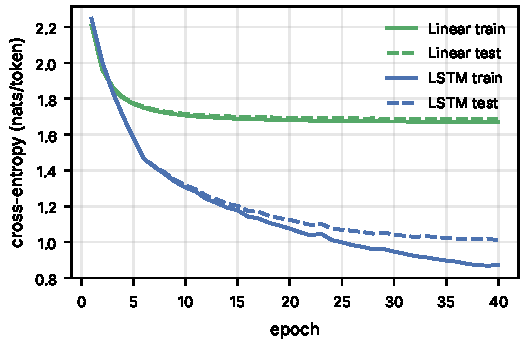
\includegraphics[width=\columnwidth]{training_curves_report.pdf}
\caption{Per-epoch cross-entropy on the training and test sets (evaluation mode).}
\label{fig:curves}
\end{figure}

\begin{table}[t]
\caption{Next-token prediction on the test set (53{,}108 targets)}
\label{tab:ce}
\centering
\begin{tabular}{lrrr}
\toprule
Model & Params & CE (nats) & Perplexity \\
\midrule
Unigram (reference) & 46 & 3.079 & 21.73 \\
Bigram Markov & 2{,}208 & 2.348 & 10.46 \\
Linear, $K{=}8$ & 18{,}480 & 1.687 & 5.40 \\
LSTM & 506{,}928 & \textbf{1.010} & \textbf{2.75} \\
\bottomrule
\end{tabular}
\end{table}

\begin{table}[t]
\caption{Statistics of 300 sampled sequences per model (fractions)}
\label{tab:gen}
\centering
\setlength{\tabcolsep}{3.2pt}
\begin{tabular}{lcccccc}
\toprule
Source & Valid & Bar fit & Scale & Closure & TV int. & Rep-4 \\
\midrule
Test data & 1.000 & 1.000 & 1.000 & 1.000 & 0.000 & 0.045 \\
Bigram, $T{=}1$ & 0.990 & 0.130 & 0.812 & 0.031 & 0.478 & 0.038 \\
Linear, $T{=}1$ & 0.877 & 0.160 & 0.869 & 0.153 & 0.025 & 0.033 \\
LSTM, $T{=}0.7$ & 0.993 & 0.990 & 0.992 & 0.667 & 0.062 & 0.006 \\
LSTM, $T{=}1.0$ & 0.980 & 0.917 & 0.980 & 0.540 & 0.029 & 0.002 \\
LSTM, $T{=}1.3$ & 0.853 & 0.742 & 0.967 & 0.445 & 0.044 & 0.001 \\
\bottomrule
\end{tabular}
\end{table}

Table~\ref{tab:gen} separates what each model captures. The bigram chain almost always obeys
the note--duration grammar, a first-order constraint, but its absolute-pitch transitions
produce wrong interval statistics (TV 0.478) and it rarely fills bars. The linear model matches
interval statistics but cannot track position within the bar (bar fit 0.160). The LSTM keeps
91.7\% of samples bar-aligned at $T{=}1.0$, and on average 98.0\% of a sample's notes lie in one scale. Lower
temperature raises validity and tonal closure; higher temperature lowers both. Two gaps
remain at every temperature: tonal closure stays well below the data (0.54 vs.\ 1.00 at
$T{=}1.0$), and motif repetition is much lower than in the data (0.002 vs.\ 0.045). No sample
from any model was an exact copy of a training piece.

For the music artifact we fixed a selection rule before listening: sample LSTM candidates at
$T{=}1.0$ with seed 2026 and keep the first that is grammatically valid, bar-aligned,
30--60\,s long at 90\,BPM, and not a training copy. The first candidate passed (23 of 50 did).
It was written to \texttt{generated\_piano.mid} (Acoustic Grand Piano, 90\,BPM, velocity 80,
notes held for 95\% of their value): 51 notes, 31.9\,s, MIDI 62--84, with no overlapping or
zero-length notes, plus a FluidSynth WAV rendering. Both are qualitative examples only.

\section{Discussion and Limitations}
The LSTM's advantage over the linear model is largest on metrical structure, which needs a
running count of elapsed time that a fixed window of eight tokens cannot hold. Its weaknesses
are long-range: returning to the opening motif and closing on the tonic depend on context
from many bars earlier. Since the train--validation gap widens after epoch 20, bar-position tokens or attention seem
more promising than extra capacity. Limitations: the data is synthetic and simple, so results do not
transfer to real piano repertoire; there is no polyphony, dynamics or expressive timing; each
model was trained once with one seed, so run-to-run variance is unmeasured; and all metrics
measure conformity to the generator, not musical value.

\section{Conclusion}
On procedurally generated melodies, a 0.5\,M-parameter LSTM clearly outperforms linear and
Markov baselines in held-out likelihood and produces mostly valid, bar-aligned, diatonic
samples. It captures local rules well but reproduces phrase-level form only partly. All data,
models, metrics and the generated MIDI are produced by one seeded Python script.

\bibliographystyle{IEEEtran}
\begin{thebibliography}{6}
\bibitem{hochreiter1997}
S.~Hochreiter and J.~Schmidhuber, ``Long short-term memory,'' \emph{Neural Comput.}, vol.~9,
no.~8, pp.~1735--1780, 1997.
\bibitem{eck2002}
D.~Eck and J.~Schmidhuber, ``Finding temporal structure in music: Blues improvisation with
LSTM recurrent networks,'' in \emph{Proc. IEEE Workshop Neural Netw. Signal Process. XII},
2002, pp.~747--756.
\bibitem{oore2018}
S.~Oore, I.~Simon, S.~Dieleman, D.~Eck, and K.~Simonyan, ``This time with feeling: Learning
expressive musical performance,'' arXiv:1808.03715, 2018.
\bibitem{briot2020}
J.-P. Briot, G.~Hadjeres, and F.-D. Pachet, \emph{Deep Learning Techniques for Music
Generation}. Cham, Switzerland: Springer, 2020.
\bibitem{srivastava2014}
N.~Srivastava, G.~Hinton, A.~Krizhevsky, I.~Sutskever, and R.~Salakhutdinov, ``Dropout: A
simple way to prevent neural networks from overfitting,'' \emph{J. Mach. Learn. Res.},
vol.~15, pp.~1929--1958, 2014.
\bibitem{kingma2015}
D.~P. Kingma and J.~Ba, ``Adam: A method for stochastic optimization,'' in \emph{Proc. Int.
Conf. Learn. Represent. (ICLR)}, 2015.
\end{thebibliography}

\end{document}
